
\documentclass[journal]{IEEEtran}
% \documentclass[journal]{../sty/IEEEtran}
\usepackage{amsmath}
\usepackage{stfloats}
\usepackage{graphicx}
\usepackage{siunitx}
\usepackage{physics}
\usepackage{listings}
\usepackage[framed,numbered,autolinebreaks,useliterate]{mcode}
\usepackage{booktabs}
\lstset{language=matlab, frame=single, breaklines, columns=flexible}
\usepackage[caption=false]{subfig}
\usepackage{url}

\begin{document}

\title{Engineering Electromagnetic Field \\ Experiment 2 Report: Distribution of Electric Field \\ Built by Continuous Line Charge}

\author{Guanchao~Huang,~Southern University of Science and Technology,~11912309@mail.sustech.edu.cn
    \thanks{with Assistant Professor Youwei Jia, and the Department of Electrical  and Electronic Engineering.}%
    \thanks{Tutorial assistant and all classmates.}}%


\markboth{IEEE Transactions on Education,~Vol.~X, No.~X, November~2020}%
{Huang: Engineering Electronics Experiment 2 Report: Distribution of Electric Field}
\maketitle


\begin{abstract}
    This experiment calculates the distribution of electric field built by continuous line charge, and plot the relevant figures on MATLAB environment. Such exercise also helps us to study the difference between integration and infinitesimal methods on analyzing electric field.
\end{abstract}


\begin{IEEEkeywords}
    IEEEtran, electric field, engineering, \LaTeX.
\end{IEEEkeywords}


\section{Introduction}

\IEEEPARstart{T}{his} experiment is for us to get used to the workflow of academic paper writing, and also having a deeper understanding on the distribution of electric field.

The complete resources of this experiment, including figures, .tex and .m source files can be retrieved at my GitHub repo: https://github.com/SamuelHuang2019/EEF-lab.


\section{Related Knowledge}

In vacuum, the electric field intensity $\mathbf{E}$ of a point charge can be expressed as:

\begin{equation}\label{e1}
    \mathbf{E} = k\frac{Q}{R^2}\mathbf{a}_R
\end{equation}

Where the coefficient $k = \SI[per-mode=symbol]{9e9}{\farad\per\meter}$ is the electrostatic constant. $Q$ represents the total amount of charge. $R$ denotes the distance between the point in the electric field and the source charge.

If we take the reference point as the infinite distance, then the electric potential at a point in the field is expressed as:

\begin{equation}\label{e2}
    V =
    k\frac{Q}{R}
\end{equation}

The electric field intensity can be expressed as the negative gradient of the electric potential.

\begin{equation}\label{e3}
    \mathbf{E} = -\nabla V
\end{equation}

The electric field generated by $N$ point charge in the vacuum is expressed as:

\begin{equation}\label{e4}
    V = \sum_{i=1}^N k\frac{Q_i}{R_i}
\end{equation}

Similarly, the field magnitude generated by $N$ point charges in the vacuum can be obtained through equation \eqref{e3}.

When the field source is continuous charge, e.g. line charge, we can readily resolve it by using infinitesimal or integral method. The procedure of applying this method is listed as follows:

\begin{enumerate}
    \item Divide the line charge into small segments of charges (usually being divided evenly).\label{item:divide}
    \item Treat each small segment of charges as a point charge and calculate the electric potential through \eqref{e2}.
    \item Sum up all the electric potential by using \eqref{e4} to obtain the electric potential.
    \item Calculate the electric field intensity generated by this line charge through \eqref{e3}.
\end{enumerate}

There exists a difference between the obtained result by infinitesimal method and the real value. The difference is determined by the number of segments we divided in step \ref{item:divide}. Generally, the more segments we take, the smaller the deviation will be. In some cases, we can also apply integration method to calculate the real distribution of the electric field, which makes it possible to study the relationship between the number of segments we divide and the deviations caused by the infinitesimal method.


\section{Experimental Contents}

Analyze the electric field distribution of line charge in a 2-D rectangular coordinate through MATLAB.

Suppose there is a uniformly distributed line charge between point $A(-1,\,0)$ and point $B(1,\,0)$, with line charge density of $\rho = \SI[per-mode=symbol]{1e-9}{\coulomb\per\meter}$. (The unit for the coordinate is \si\meter)

\subsection{Electric Potential Distribution Calculation by Integral}

Using integration method to calculate the distribution of electric potential at each point of the coordinate, namely, the real distribution. The procedure is given below:

Given a point $(X_0,\, Y_0)$.

\begin{equation}
    \begin{aligned}
        V & =
        k\int_{-1}^1 \frac{\rho\dd{x}}{R}                                           \\ & =
        k\int_{-1}^1 \frac{\rho\dd{x}}{\sqrt{(x - X_0)^2 + Y_0^2}}                  \\ & =
        k\rho\ln\left.\left|(x-X_0) + \sqrt{(x-X_0)^2 + Y_0^2}\right|\right|_{-1}^1 \\ & =
        k\rho\ln\left[
            \frac{1 - X_0 + \sqrt{(1-X_0)^2 + Y_0^2}}{-1-X_0 + \sqrt{(-1-X_0)^2 + Y_0^2}}
            \right]
    \end{aligned}
\end{equation}

The range for the points considered is from $-5$ to $5$, on both $x$ and $y$ directions. The coordinate plane then is evenly divided in to a $50$ by $50$ mesh grid.

\begin{figure}[hbtp]
    \centering
    \subfloat[Potential distribution]{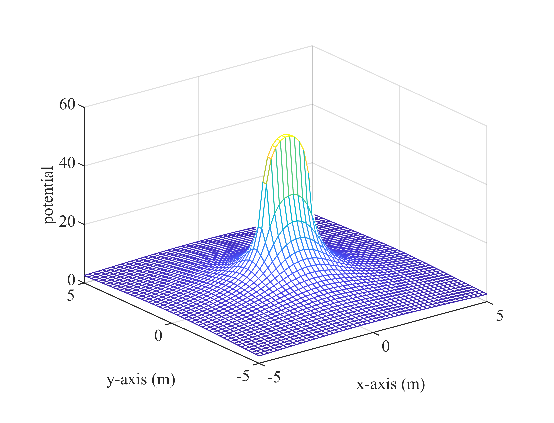
\includegraphics[width=88mm]{huang1}%
        \label{fig:potential_int}} \\
    \subfloat[Potential contours]{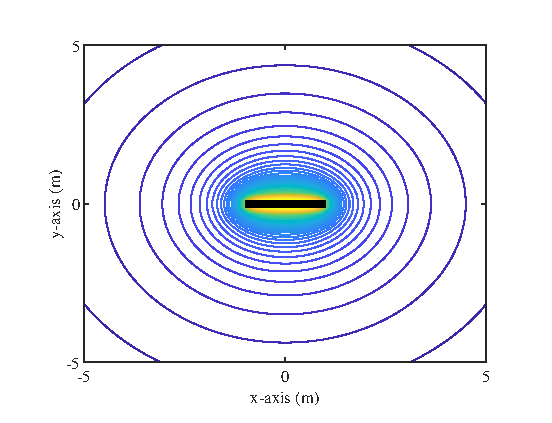
\includegraphics[width=88mm]{huang2}%
        \label{fig:contours_int}} \\
    \subfloat[Electric field lines]{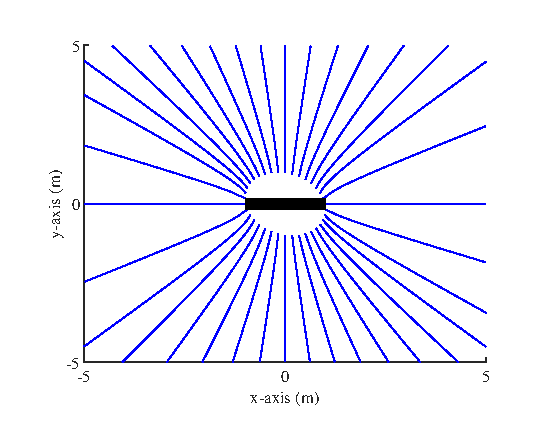
\includegraphics[width=88mm]{huang3}%
        \label{fig:field_int}}
    \caption{Potential distribution obtained by integration.}
    \label{fig:integral}
\end{figure}

\begin{lstlisting}
k = 9e9;
rho = 1e-9;

xm = 5;
ym = 5;
x = linspace(-xm, xm, 50);
y = linspace(-ym, ym, 50);
[X, Y] = meshgrid(x, y);
V = k * rho * log((1 - X + sqrt((1 - X).^2 + Y.^2)) ./ (-1 - X + sqrt((-1 - X).^2 + Y.^2)));

mesh(X, Y, V)
\end{lstlisting}

According to the plot of the potential distribution, in the contours we can consider the minimum of \SI{0}{\volt} and the maximum of \SI{50}{\volt}, equally divided into 50 equipotential lines.

\begin{lstlisting}
Vmin = 0;
Vmax = 50;
Veq = linspace(Vmin, Vmax, 50);

figure
(X, Y, V, Veq);
hold on
plot([-1, 1], [0, 0], 'k', 'LineWidth', 3)
\end{lstlisting}

Once the potential distribution is obtained, the electric field lines can be easily plotted by taking negative gradient.

\begin{lstlisting}
[Ex, Ey] = gradient(-V);
figure
streamline(X, Y, Ex, Ey, xs, ys)
hold on
plot([-1, 1], [0, 0], 'k', 'LineWidth', 5)
\end{lstlisting}


\subsection{Electric Potential Distribution Calculation by Infinitesimal Method}

For the infinitesimal method, the key is to sum the potential due to all the segments. The procedures of calculating potential distribution and generate figures are encapsulated in function segments.

\begin{lstlisting}
function V = segments(n)

    global k
    global rho
    global X
    global Y
    global Veq
    global xs
    global ys

    Q = rho * 2 / n;
    d = 2 / n;
    V = zeros(50, 50);

    for index = 1:n
        V = V + k * Q ./ sqrt((X - (-1 + d * index)).^2 + Y.^2);
    end

    figure
    mesh(X, Y, V)

    figure
    contour(X, Y, V, Veq);
    hold on
    plot([-1, 1], [0, 0], 'k', 'LineWidth', 3)

    [Ex, Ey] = gradient(-V);
    figure
    streamline(X, Y, Ex, Ey, xs, ys)
    hold on
    plot([-1, 1], [0, 0], 'k', 'LineWidth', 5)

end
\end{lstlisting}

Basic variables are defined globally, line 11 and 12 calculates the amount of charge and length. The potential due to each segment of charged lines is summed within a for loop. The rest part of the function is just the same as for the integral method.

\begin{figure}[!hbtp]
    \centering
    \subfloat[Potential distribution]{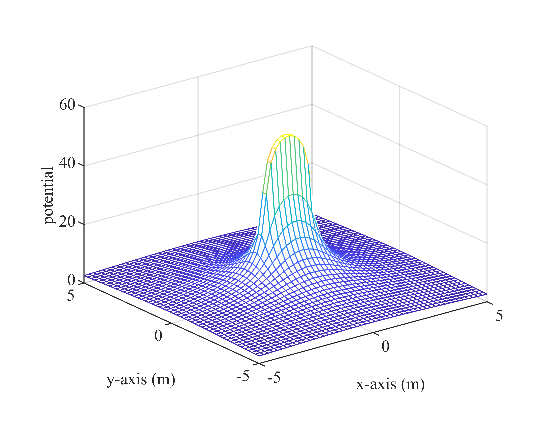
\includegraphics[width=88mm]{huang4}%
        \label{fig:potential_20}} \\
    \subfloat[Potential contours]{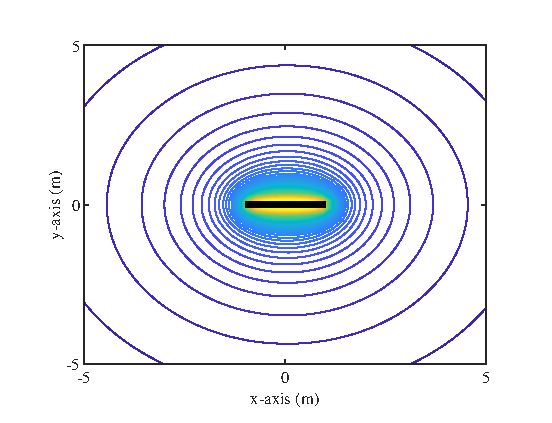
\includegraphics[width=88mm]{huang5}%
        \label{fig:contours_20}} \\
    \subfloat[Electric field lines]{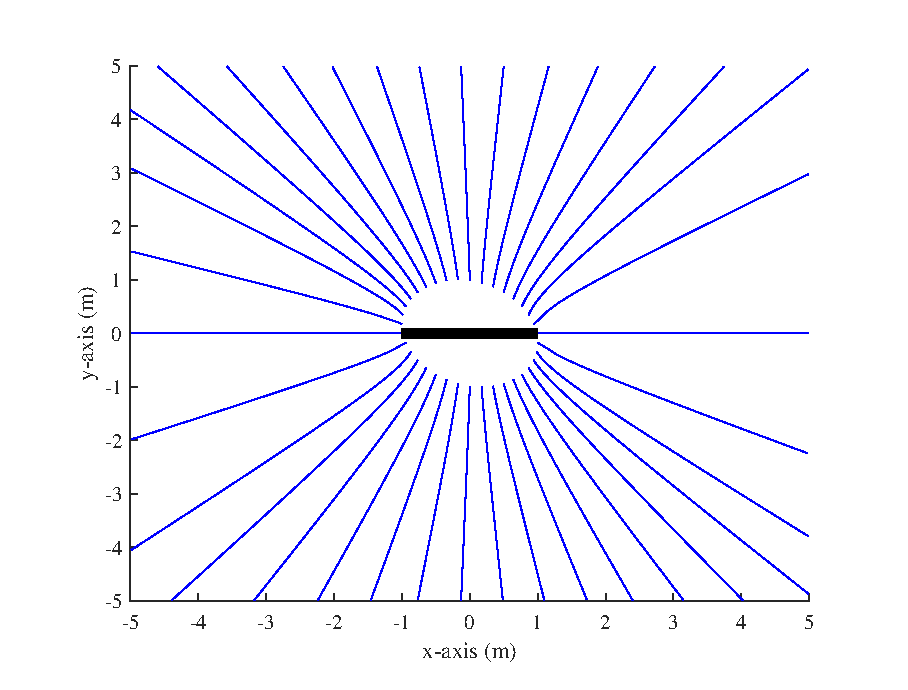
\includegraphics[width=88mm]{huang6}%
        \label{fig:field_20}}
    \caption{Potential distribution obtained by infinitesimal method, divided into 20 segments.}
    \label{fig:infinitesimal_20}
\end{figure}

\begin{figure}[!hbtp]
    \centering
    \subfloat[Potential distribution]{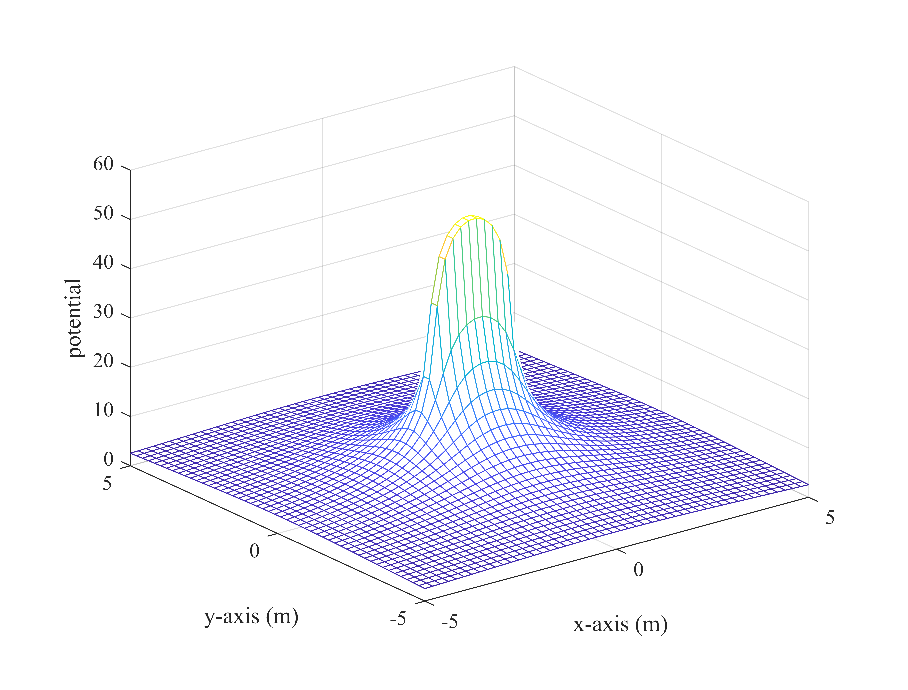
\includegraphics[width=88mm]{huang7}%
        \label{fig:potential_50}} \\
    \subfloat[Potential contours]{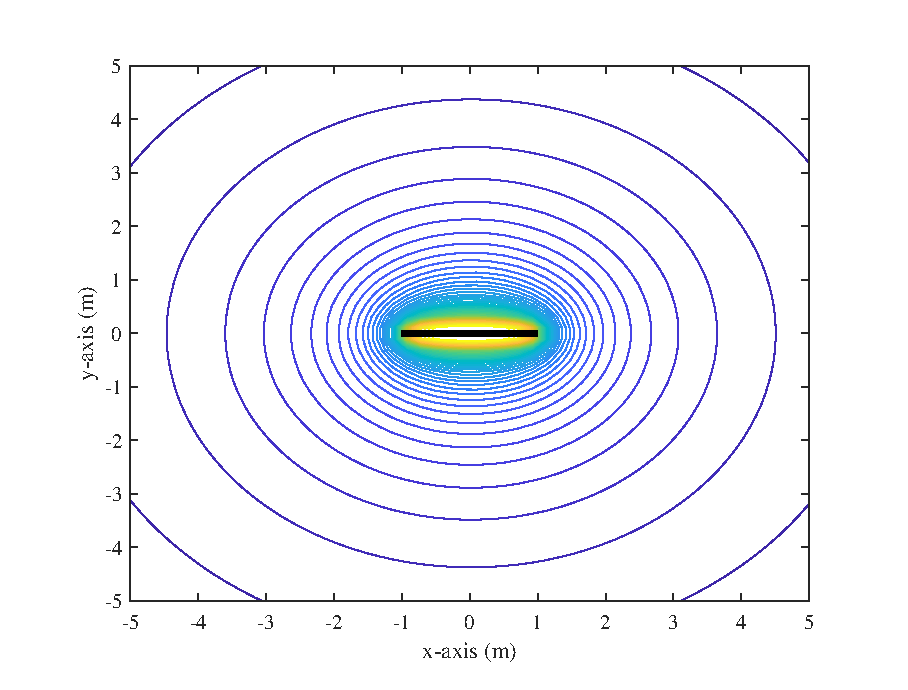
\includegraphics[width=88mm]{huang8}%
        \label{fig:contours_50}} \\
    \subfloat[Electric field lines]{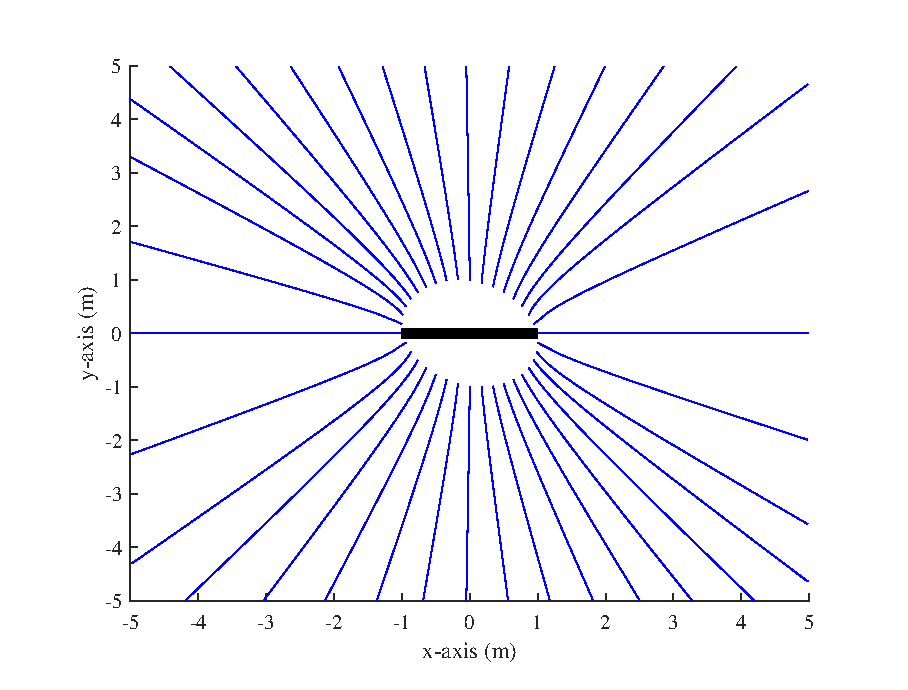
\includegraphics[width=88mm]{huang9}%
        \label{fig:field_50}}
    \caption{Potential distribution obtained by infinitesimal method, divided into 50 segments.}
    \label{fig:infinitesimal_50}
\end{figure}

\begin{figure}[!hbtp]
    \centering
    \subfloat[Potential distribution]{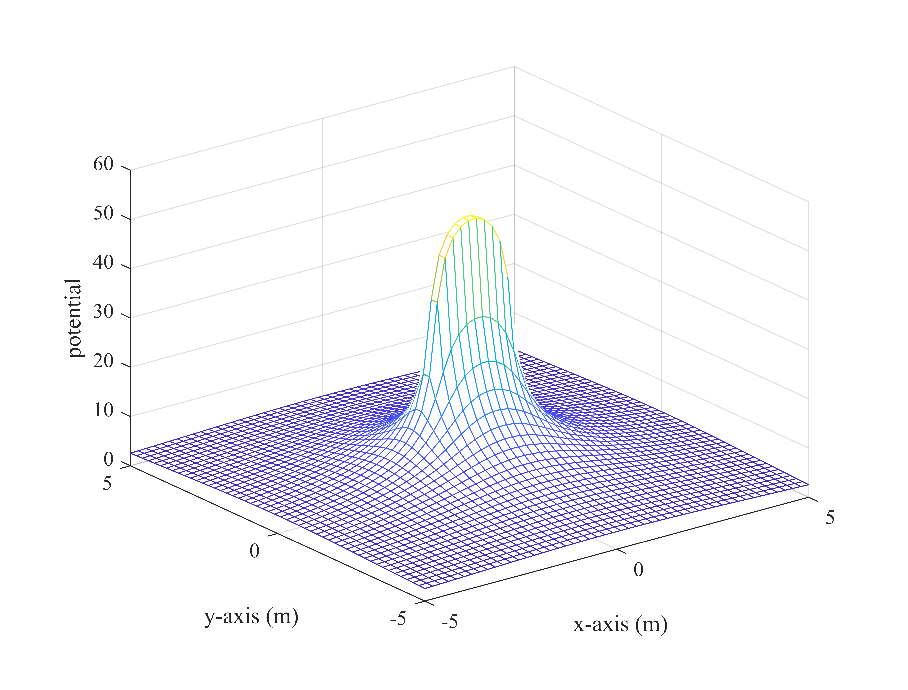
\includegraphics[width=88mm]{huang10}%
        \label{fig:potential_100}} \\
    \subfloat[Potential contours]{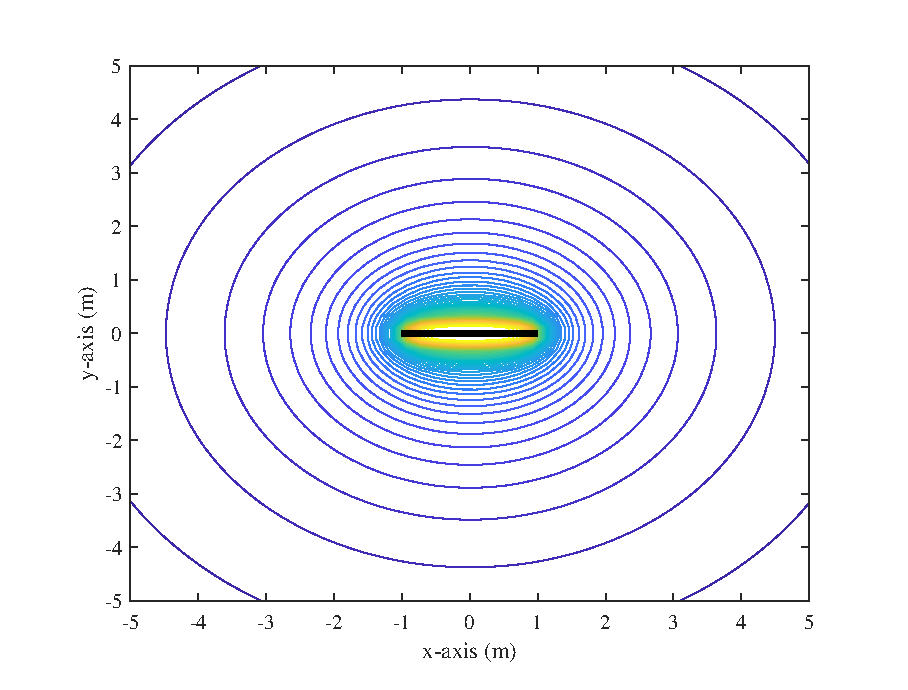
\includegraphics[width=88mm]{huang11}%
        \label{fig:contours_100}} \\
    \subfloat[Electric field lines]{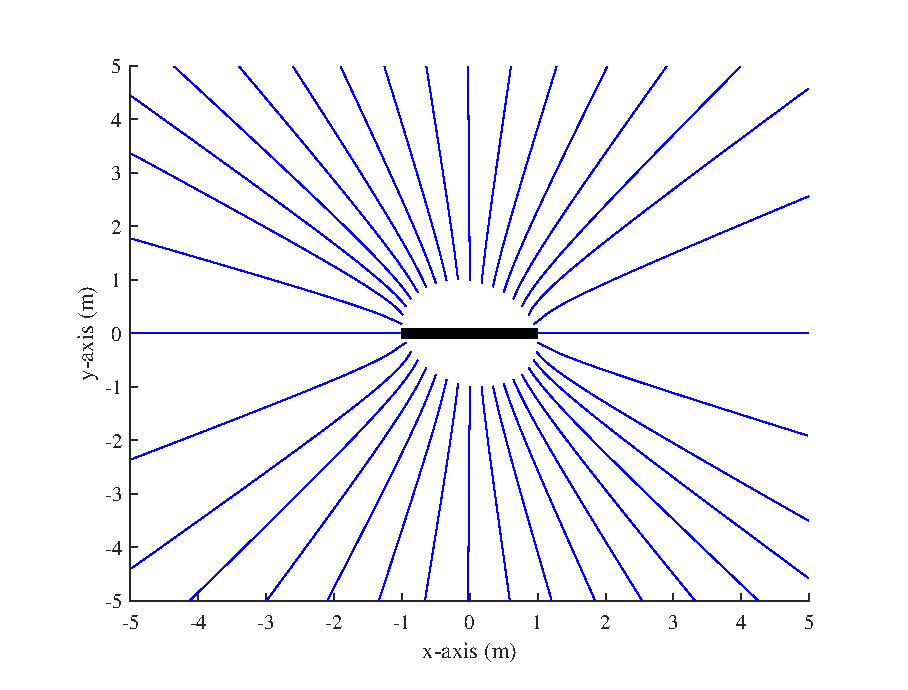
\includegraphics[width=88mm]{huang12}%
        \label{fig:field_100}}
    \caption{Potential distribution obtained by infinitesimal method, divided into 100 segments.}
    \label{fig:infinitesimal_100}
\end{figure}

By calling this function, we can obtain the potential distribution and its plot calculated with different numbers of segments.

\begin{lstlisting}
V20 = segments(20);
V50 = segments(50);
V100 = segments(100);
\end{lstlisting}

According to Figure \ref{fig:infinitesimal_20}, Figure \ref{fig:infinitesimal_50} and Figure \ref{fig:infinitesimal_100}, compared with Figure \ref{fig:integral}, it is apparent that the plot generated by integral method and infinitesimal method, even with only 50 segments, can not be distinguished with unaided eyes.

\subsection{Comparison Between Integral and Infinitesimal Method}

Since human eyes can not tell the difference between infinitesimal and integral method, I analysed the two methods statistically.

\begin{lstlisting}
Vd20 = abs(V - V20);
Vd50 = abs(V - V50);
Vd100 = abs(V - V100);

figure
mesh(X, Y, Vd20)
figure
mesh(X, Y, Vd50)
figure
mesh(X, Y, Vd100)

d20 = sum(sum(Vd20.^2)) / (50 * 50);
d50 = sum(sum(Vd50.^2)) / (50 * 50);
d100 = sum(sum(Vd100.^2)) / (50 * 50);
\end{lstlisting}

Qualitatively, Figure \ref{fig:difference} shows the absolute value of difference between potential obtained with integral and infinitesimal method at each point. We can see from the $z$-axis that, the more the segments are divided into, the smaller the difference between the integral method and the infinitesimal method is. What's more, the biggest difference appears at the two ends of the charged line.

\begin{figure}[hbtp]
    \centering
    \subfloat[Divided into 20 segments]{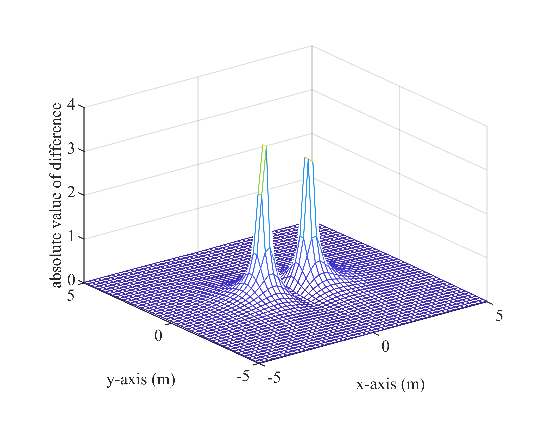
\includegraphics[width=88mm]{huang13}%
        \label{fig:difference_20}} \\
    \subfloat[Divided into 50 segments]{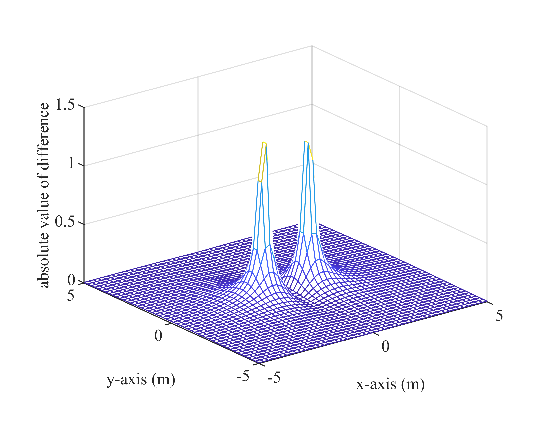
\includegraphics[width=88mm]{huang14}%
        \label{fig:difference_50}} \\
    \subfloat[Divided into 100 segments]{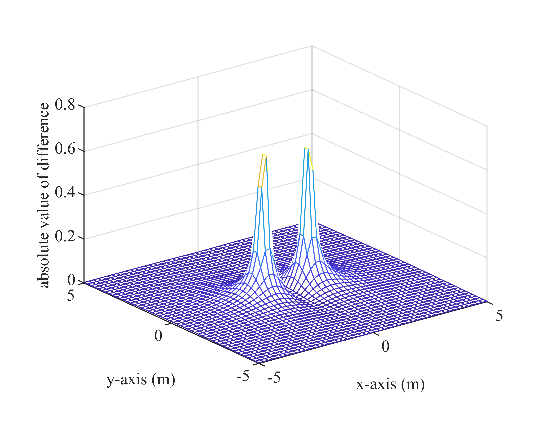
\includegraphics[width=88mm]{huang15}%
        \label{fig:difference_100}}
    \caption{Absolute value of difference between potential obtained with integral and infinitesimal method at each point}
    \label{fig:difference}
\end{figure}

Quantitatively, we can calculate the deviation between the integral method and the infinitesimal method. In this case, as in table \ref{tab:deviation} shows, the more segments are divided into, the smaller the deviation is. For 100 segments with respect to 20 segments, this value decreases to one twenty-fifth.

\begin{table}[h]
    \renewcommand{\arraystretch}{1.3}
    \caption{the Deviation Between the Potential Distribution Obtained from Integral and the Infinitesimal Method}
    \label{tab:deviation}
    \centering
    \begin{tabular}{c|ccc}
        \toprule
        \textbf{segments}  & 20     & 50     & 100    \\
        \hline
        \textbf{deviation} & 0.0507 & 0.0081 & 0.0020 \\
        \bottomrule
    \end{tabular}
\end{table}

\section{Conclusion}

Through this experiment, we obtained these facts:

\begin{itemize}
    \item The difference between the potential distribution obtained from integral and infinitesimal method, when divided into over 20 segments, can be distinguished through plot with unaided eyes.
    \item The maximum difference occurs at around the two ends of the charged line.
    \item The more the segments are divided into, the smaller the difference is.
\end{itemize}

Based on this, in most cases, infinitesimal method is good enough for evaluating the potential distribution. However, when considering near the ends of the charged line, we will need to make more rigorous and concise calculation.


\ifCLASSOPTIONcaptionsoff
    \newpage
\fi


\begin{thebibliography}{1}

    \bibitem{IEEEhowto:kopka}
    H.~Kopka and P.~W. Daly, \emph{A Guide to \LaTeX}, 3rd~ed.\hskip 1em plus
    0.5em minus 0.4em\relax Harlow, England: Addison-Wesley, 1999.
    \bibitem{EE:hayt}
    W.~H. Hayt, Jr. and J.~A. Buck, \emph{Engineering Electromagnetics}, 8th~ed.\hskip 1em plus
    0.5em minus 0.4em\relax New York, USA: McGraw-Hill, 2012.

\end{thebibliography}


\begin{IEEEbiography}[{\includegraphics[width=1in,height=1.25in,clip,keepaspectratio]{huang.png}}]{Guanchao Huang}

    was born in Linwu County, Chenzhou, Hunan Province, China in 2002. He received the junior middle school degree from the Third Middle School of Linwu, in 2016 and the senior middle school degree from the First High School of Chenzhou in 2019.

    Since 2019, he has been an undergraduate student with the School of Microelectronics, Southern University of Science and Technology, Shenzhen, Guangdong Province, China. He is the author of two experiment reports on  engineering electromagnetic field.

\end{IEEEbiography}


\end{document}


